\section{The Flyspeck Project}
\label{sec:flyspeck}

\begin{wrapfigure}{r}{4.2cm}
  \centering
  \vspace{-.95cm}
  \begin{tikzpicture}
    \node (s) at (0,0) {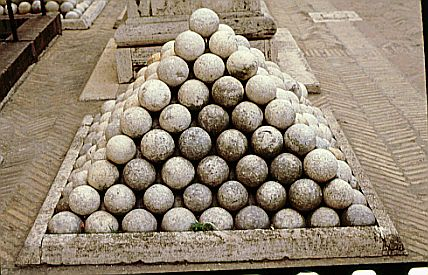
\includegraphics[width=4cm]{images/cannonballs.jpg}};
    \node at (s.south) {\raisebox{-2ex}{\scriptsize (http://tinyurl.com/3bxx2t)}};
  \end{tikzpicture}
  \vspace{-1.0cm}
  \caption{The face centered cubic packing}
  \vspace{-1.0cm}
\end{wrapfigure}

%% alternative images are
%% http://cosmicadventure.com/gallery/albums/album48/Cannonballs_2.jpg
%% http://mathworld.wolfram.com/images/eps-gif/CircleSpherePacking_800.gif
%% http://en.wikipedia.org/wiki/Image:Close-packed_spheres.jpg

The target of our case study is the Flyspeck Project, which seeks to
formally verify Thomas Hales' 2005 proof of the Kepler Conjecture.
The Kepler Conjecture asserts that the density of a packing of unit
spheres in 3 dimensions is at most $\pi/(3\sqrt{2})$, the density of the face centered
cubic and hexagonal close packings.  The conjecture, posed by Kepler
in 1611, formed part of Hilbert's 18th problem, and until its solution
was recognized as one of the most famous unsolved problems of
mathematics.

Hales' proof, completed in 1995, was not accepted immediately by the
mathematical community.  Besides its considerable length, the proof relies
essentially on computer calculations.  The 300 pages of text and many thousands
of lines of computer code made checking the proof for errors in the referee
process unusually difficult, leading to a publication delay of nearly 10 years.
In 2003, Hales proposed using computers to rigorously check the entire proof in
detail, including the computer code.  He dubbed this effort the \textit{Flyspeck
  Project}\footnote{The word ``flyspeck'' means, ``to examine closely''.  It was
  found by Hales using a regular expression search of an English dictionary for
  the expression ``F.*P.*K'', for ``Formal Proof of Kepler''}.  The software
systems used in such formalizations are called \textit{theorem provers} or
\textit{proof assistants}.  Beginning with a set of axioms and inference rules,
they can, with adequate human guidance, verify that a purported proof follows
from the axioms.  Examples of proof assistants are
Isabelle\cite{Paulson:1994:Isabelle}, Coq\cite{Bertot:2004:CoqBook}, and HOL
Light\cite{Harrison:2000:HOL-Light}. (The word ``formalize'' is used in many
contexts in this field.  In the remainder of this paper, we use ``formal'' and
``formalize'' loosely, possibly referring to any degree of colloquial or
scientific formalization.  We use use ``computerized'' to mean that a theorem,
proof or definition has been expressed in a proof assistant.  Note that we
consider computerized definitions and proofs ``documents'' in the sense of
section \ref{sec:science}.)

  Unfortunately, modern proof assistants are still far from being able to check
proofs at the level given in most journals and mathematics textbooks.  A typical
estimate is that it takes about a week to formalize a single page of mathematical
text.  Based on such estimates, Hales expects that it will take 
around 20 man-years to complete the Flyspeck project.  
Hales is compiling a book\cite{Hales:2007:FlyspeckBook}
of lemmas from different areas of mathematics that are needed in his proof. 
That book is currently 450 pages, and contains a significant percentage
of the mathematical results used in the proof.  It covers such disperate topics
as plane, solid, and sphereical geometry, graph theory and hypermaps, single and
multivariable calculus, and plane and sphereical trigonometry.

The first steps toward a computerized proof have already been taken.
Nipkow and Bauer\cite{Nipkow:2005:Tame} proved the correctness of a
fundamental algorithm in Isabelle.  The other two main parts of the
computer code, linear programming and global optimization, are
currently being investigated in doctoral
dissertations\cite{Zumkeller:2006:TaylorModels,Obua:2005:LinearPrograms}.
There is a project page\cite{website:FlyspeckProjectPage} for Flyspeck
that documents some of this progress.  That page has a source
repository containing the book of lemmas, as well as the formalized
definitions of some important functions and inequalities.  

Thus, while
considerable progress has been made on the computer code, the bulk of
the mathematical formalization remains to be done.  This formalization
will consist of two broad phases.  First, a number of elementary
mathematical theories (e.g. spherical geometry) need to be defined and
the relevant lemmas proved.  Then the specific aspects of the Kepler
proof that relies on the elementary results need to be formalized.
Given the content of the book mentioned above, we suspect that
Flyspeck, in its final form, will consist of dozens of theories, with
hundreds of definitions and thousands of lemmas.

Flyspeck is particularly appealing as a use case for a semantic wiki
approach. While the ultimate result is to be a highly formal
computerized proof, the current proof involves both highly formal and
semi-formal mathematical knowledge.  It contains descriptive and
motivating yet informal text that should be preserved for human
understanding.  This quasi-formal information would be difficult to
present in a strictly formal setting of a proof assistant, but is at
home in a semantic wiki.  The large number of lemmas, many independent
or only loosely coupled, suggest a ``crowdsourcing'' approach will be
beneficial. Thus we anticipate that a semantic wiki for organizing the
collaboration will be ideal.  For example, presenting the progress on
the web will contribute to communicating which parts of the proof are
already computerized, and which remain to be done.  Finally, its
ultimate purpose is to develop a large scientific document and to
communicate this document to the public, a proven strength of 
the wiki medium.

%%% Local Variables: 
%%% mode: latex
%%% TeX-master: "flyspeck-wiki-eswc08"
%%% End: 
